\subsection{Methodology}

In this section we will briefly describe the methodology we have chosen 
for this project. We will also described how the methodology works and 
how we have adapted the methodology in to the project.
The prestudy on why we have chosen Scrum is described 
under the 'preliminary studies'. 

{\bf What is a methodology? } A project methodology is a approach a project can take to manage all the project activites. There are several types of approaches to take like iterative, incremental, sequential, etc. Regardless of the approach, every project has activites to complete, but it can be scheduled differently. 

{\bf What is a agile methodology? } In a 'normal' project cycle we have activites like analysis, planning, implementation, testing and delivery. How a project schedule these activites depends on the approach. 
The agile approache focus on helping the team to respond to unpredictability through incremental, iterative work cadences, known as sprints/pahses. Agile methodologies are an alternative to waterfall, or traditional sequential development.
Agile development has a known manifest called 'The agile manifesto' that works like this:

\begin{itemize}
	\item Individuals and interactions over processes and tools
    \item Working software over comprehensive documentation
    \item Customer collaboration over contract negotiation
    \item Responding to change over following a plan 
\end{itemize}

The agile manifesto is based on twelve principle that is inportant to understand before
adapting a agile methodology to the project:

\begin{enumerate}
    \item Customer satisfaction by rapid delivery of useful software
    \item Welcome changing requirements, even late in development
    \item Working software is delivered frequently (weeks rather than months)
    \item Working software is the principal measure of progress
    \item Sustainable development, able to maintain a constant pace
    \item Close, daily cooperation between business people and developers
    \item Face-to-face conversation is the best form of communication (co-location)
    \item Projects are built around motivated individuals, who should be trusted
    \item Continuous attention to technical excellence and good design
    \item Simplicity—the art of maximizing the amount of work not done—is essential
    \item Self-organizing teams
    \item Regular adaptation to changing circumstances
\end{enumerate}


{\bf What is scrum? } Scrum is a iterative process with focus on small deliveries and a small set of roles. 
The process defines a self-sustaining team ("The scrum team") that defines the goal for each phase. The goal 
is achived through small product increments in iteration that normally last for 1-4 weeks. 
All the functions to implement is planned and is added to a listcalled a "Product Backlog". The
functions is normally defined as userstories and is added in a prioritized order. In each inkrement, 
in scrum called a "Sprint", there is a sprint meeting where the scrum team pick userstories from the 
product backlog and add them to a "Sprint Backlog". The sprint backlog is the description of what 
to deliver in the end of the sprint.

In a scrum team there is a small set of roles. There is mainly only three roles: 
\begin{itemize}
    \item {\bf The product owner: }
    \item {\bf The scrum master: }
    \item {\bf The scrum team: }
\end{itemize}

A sprint have daily meetings calles a "standup" where all members in the scrum team stand up
to tell what they have done since last standup, what they have finished, what to do do this day and
tells about any problems if any. The meeting is a very short meeting just to give the team a status
update. The standup is 

After a sprint delivery it is normal to have a "Sprint review" and a "Sprint Retrospective".
The sprint review the team make a presentation/demonstraion to a group og stakeholders (like the
customers). The Purpose of this is to get feedback on the sprint delivery. Since the development
is done in increments, it is possible for the stakeholders to add and change the requirement as
well as the implementation done so far. A sprint review then works like small "aceptance tests", 
because the customers gets the oppertunity to say "keep doing what you are doing" or "we want to change
what you have done". In this way the stakeholders are always aware of the status and it is important
way to ensure that the stakeholders will be happy with the final prduct that is developed. 
In other methodologies, the stakeholders is not as much a part of this because there is nor a 
continous delivery, but a big delivery in the end (like in the waterfall process).

In a sprint retrospective is a meeting after the sprint review where the members talk about what 
the team should start doing, stop doing and continue doing. The purpose of this meeting is to always 
get the team to work better and more effective as a team.

{\bf The phases in a sprint: }

\begin{figure}[!ht]
    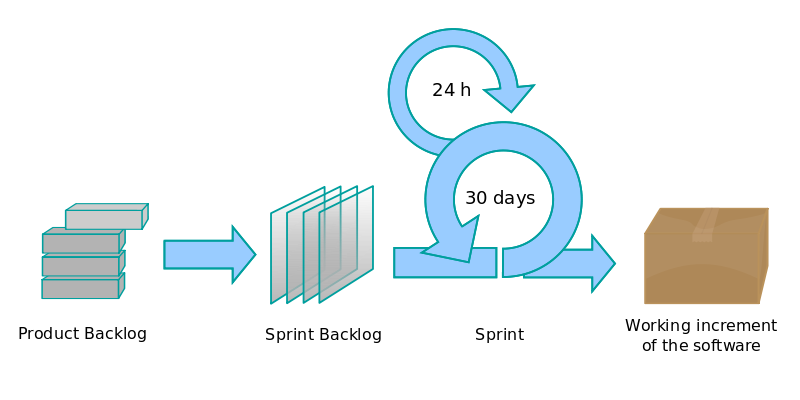
\includegraphics[scale=0.4]{pictures/Scrumprocess.png}
\end{figure}

{\bf How do we do scrum in the project? }


%http://en.wikipedia.org/wiki/Agile_software_development